\documentclass{beamer}
\usepackage[english,russian]{babel}
\usepackage[utf8]{inputenc}
\usepackage{amsmath}
\usepackage{hyperref}
\usetheme{Warsaw}
\usepackage{listings}
\usepackage{xcolor}
\usepackage{tikz}
\usetikzlibrary{graphs}
\usepackage{algpseudocode}

\lstset{
    frame=tb,
    tabsize=4,
    showstringspaces=false,
    numbers=left,
    commentstyle=\color{green},
    keywordstyle=\color{blue},
    stringstyle=\color{red},
    emph={baz},
    emphstyle=\textbf
}
\begin{document}

\title{SAT/SMT solvers\ \newline 12. Binary Decision Diagrams}
\author{Roman Kholin}
\institute{Lomonosov Moscow State University}
\date{Moscow, 2023}

\begin{frame}
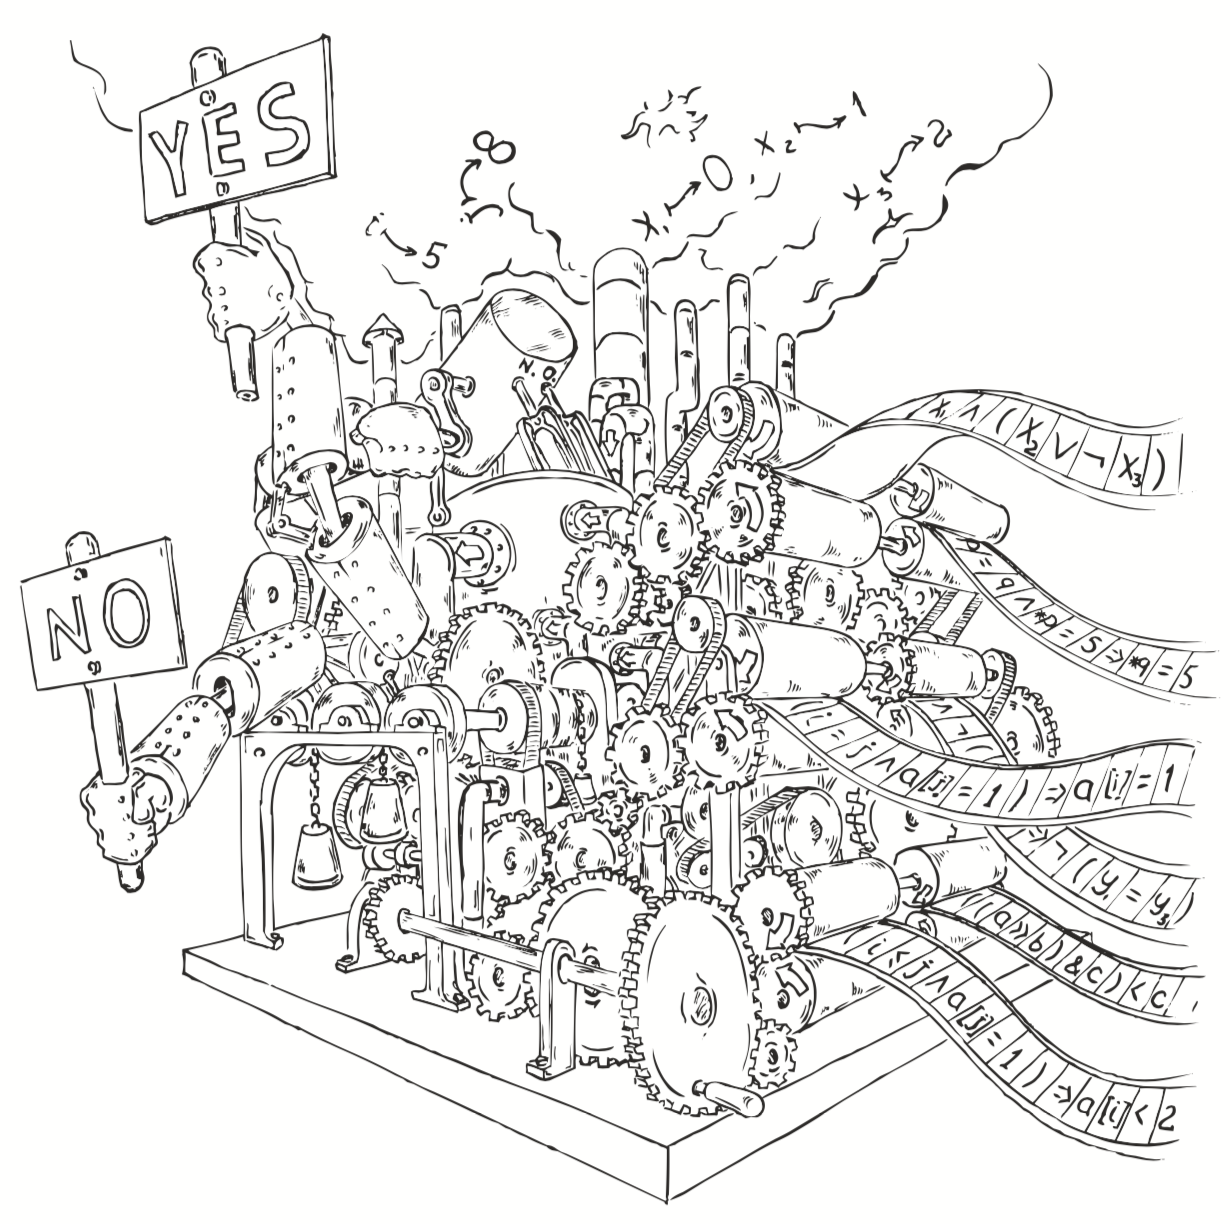
\includegraphics[scale=0.5]{../decision-procedure.png}
\end{frame}

\frame{\titlepage}

\begin{frame}{Binary Decision Trees}
A binary decision tree is a rooted, directed tree with two types of vertices, terminal vertices and nonterminal vertices.\newline
Each nonterminal vertex $v$ is labeled by a variable $var(v)$ and has two successors:\newline
\begin{itemize}
\item $low(v)$ corresponding to the case where the variable $v$ is assigned $0$
\item $high(v)$ corresponding to the case where the variable $v$ is assigned $1$
\end{itemize}
Each terminal vertex $v$ is labeled by $value(v)$ which is either $0$ or $1$
\end{frame}

\begin{frame}{Binary Decision Trees}
$f(a_1, a_2, b_1, b_2) = (a_1 \iff b_1) \wedge (a_2 \iff b_2)$
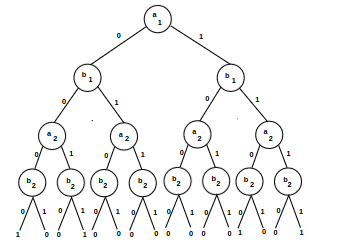
\includegraphics[scale=0.5]{decision_tree.png}\newline
There is usually a lot of redundancy in such trees\newline
There are eight subtrees with roots labeled by $b_2$, but only three are distinct\newline
\end{frame}

\begin{frame}{Binary Decision Diagrams}
\begin{itemize}
\item Binary decision diagram is a rooted, directed acyclic graph with two types of vertices, terminal vertices and nonterminal vertices
\item Each nonterminal vertex $v$ is labeled by a variable $var(v)$ and has two successors, $low(v)$ and $high(v)$
\item Each terminal vertex is labeled by either 0 or 1
\end{itemize}
\end{frame}

\begin{frame}{Example}
$f = x_1 x_2 + x_4$\newline
($x_1 \wedge x_2 \vee x_4$)
\end{frame}

\begin{frame}{Odd parity function}
$x_1 x_2 x_3 x_4$
\end{frame}

\begin{frame}{$\lnot, \vee, \wedge$}
\end{frame}

\begin{frame}{Canonical Form Property}
\begin{itemize}
\item Such a representation must guarantee that two boolean functions are logically equivalent if and only if they have isomorphic representations
\item This simplifies tasks like checking equivalence of two formulas and deciding if a given formula is satisfiable or not
\end{itemize}
Two binary decision diagrams are isomorphic if there exists a bijection $h$ between the graphs such that:
\begin{itemize}
\item terminals are mapped to terminals and nonterminals are mapped to nonterminals
\item for every terminal vertex $v$, $value(v) = value(h(v))$
\item for every nonterminal vertex $v$:
\begin{itemize}
\item $var(v) = var(h(v))$
\item $h(low(v)) = low(h(v))$
\item $h(high(v)) = high(h(v))$
\end{itemize}
\end{itemize}
\end{frame}

\begin{frame}{Canonical Form Property}
To obtain a canonical representation for boolean functions by placing two restrictions on binary decision diagrams:
\begin{itemize}
\item The variables should appear in the same order along each path from the root to a terminal
\item There should be no isomorphic subtrees or redundant vertices in the diagram
\end{itemize}
The first requirement is easy to achieve:
\begin{itemize}
\item Impose total ordering < on the variables in the formula
\item Require that if vertex $u$ has a nonterminal successor $v$, then $var(u) < var(v)$
\end{itemize}
\end{frame}

\begin{frame}{Canonical Form Property}
The second requirement is achieved by repeatedly applying three transformation rules that do not alter the function represented by the diagram:
\begin{itemize}
\item Remove duplicate terminals: Eliminate all but one terminal vertex with a given label and redirect all arcs to the eliminated vertices to the remaining one
\item Remove duplicate nonterminals: If nonterminals $u$ and $v$ have $var(u) = var(v)$, $low(u) = low(v)$ and $high(u) = high(v)$, then eliminate one of the two vertices and redirect all incoming arcs to the other vertex
\item Remove redundant tests: If nonterminal vertex $v$ has $low(v) = high(v)$, then eliminate $v$ and redirect all incoming arcs to $low(v)$
\end{itemize}
The term Ordered Binary Decision Diagram (OBDD) will be used to refer to the graph obtained in this manner
\end{frame}

\begin{frame}{Example}
\end{frame}

\begin{frame}{Ordered Binary Decision Diagrams}
\begin{itemize}
\item The canonical form may be obtained by applying the transformation rules until the size of the diagram can no longer be reduced
\item It was shown how this can be done by a procedure called Reduce in linear time
\end{itemize}
If OBDDs are used as a canonical form for boolean functions, then
\begin{itemize}
\item checking equivalence is reduced to checking isomorphism between OBDDs
\item satisfiability can be determined by checking equivalence with the trivial OBDD that consists of only one terminal labeled by 0
\end{itemize}
\end{frame}

\begin{frame}{OBDD for Comparator Example}
$a_1 < b_1 < a_2 < b_2$\newline
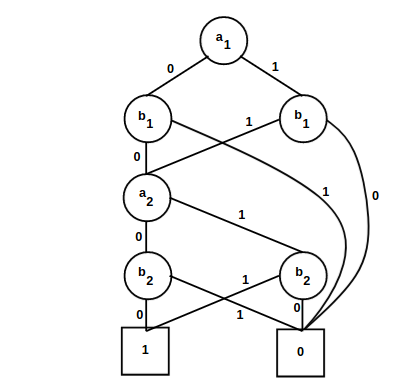
\includegraphics[scale=0.5]{comp1.png}\newline
The number of vertices will be $3n + 2$
\end{frame}

\begin{frame}{OBDD for Comparator Example}
$a_1 < a_2 < b_1 < b_2$\newline
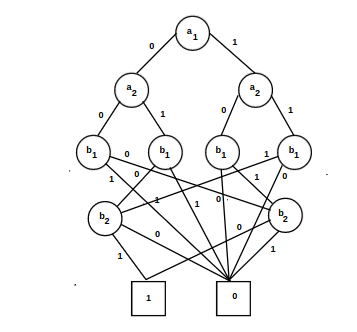
\includegraphics[scale=0.5]{comp2.png}\newline
The number of vertices will be $3*2^n - 1$
\end{frame}

\begin{frame}{Logical Operations}
How to get OBDD for $f * g$ (if we know OBDDs for f and g)?\newline
The key idea for efficient implementation of these operations is the Shannon expansion\newline
$f = \lnot x\wedge f|_{x = 0} \vee x\wedge f|_{x = 1}$\newline
Let $*$ be an arbitrary two argument logical operation, and let $f$ and $f'$ be two boolean functions\newline
To simplify the explanation of the algorithm we introduce the following notation:
\begin{itemize}
\item $v$ and $v'$ are the roots of the OBDDs for $f$ and $f'$
\item $x = var(v)$ and $x' = var(v')$
\end{itemize}
\end{frame}

\begin{frame}{Logical Operations}
\begin{itemize}
\item If $v$ and $v'$ are both terminal vertices, then $f * f' = value(v) * value(v')$
\item If $x = x'$, then we use the Shannon expansion $f * f' = \lnot x\wedge (f|_{x = 0} * f'|_{x = 0}) \vee x\wedge (f|_{x = 1} * f'|_{x = 1})$
\item If $x < x'$, then $f'|_{x = 0} = f'|_{x = 1} = f'$ since $f'$ does not depend on x. In this case the Shannon Expansion simplifies to $f * f' = \lnot x\wedge (f|_{x = 0}) \vee x\wedge (f|_{x = 1})$
\item If $x > x'$ - in the previous manner
\end{itemize}
\end{frame}

\begin{frame}{Logical Operations}
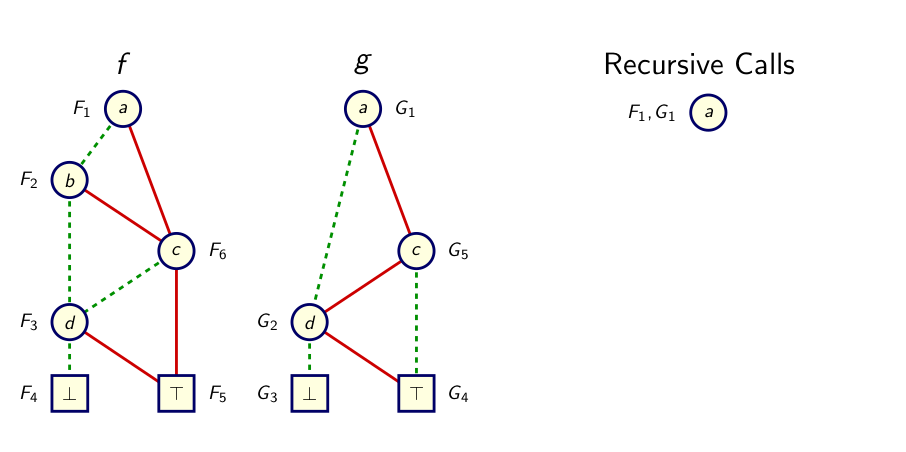
\includegraphics[scale=0.35]{ex1.png}
\end{frame}

\begin{frame}{Logical Operations}
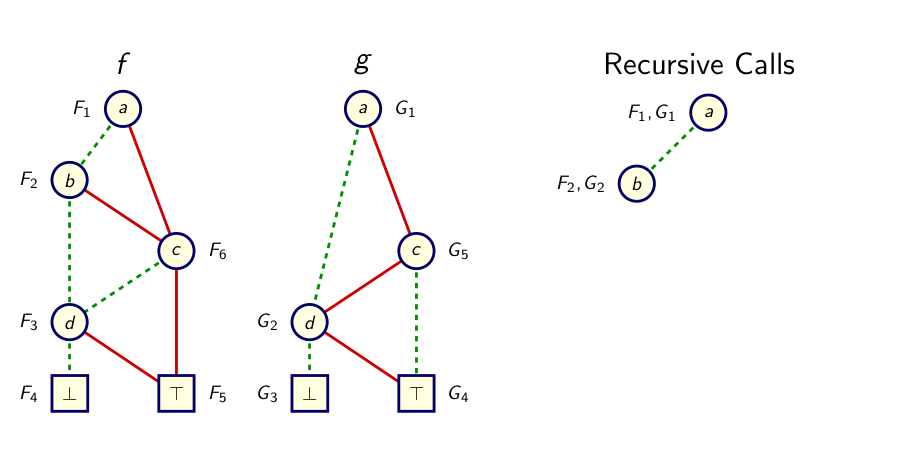
\includegraphics[scale=0.35]{ex2.png}
\end{frame}

\begin{frame}{Logical Operations}
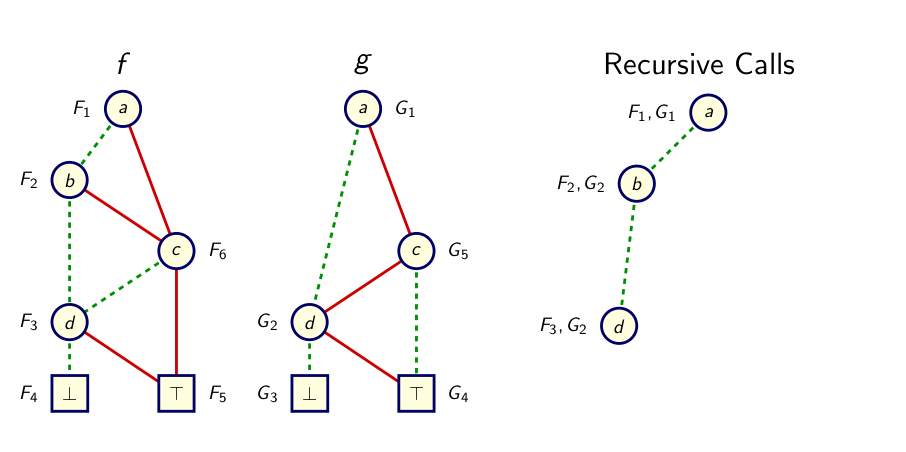
\includegraphics[scale=0.35]{ex3.png}
\end{frame}

\begin{frame}{Logical Operations}
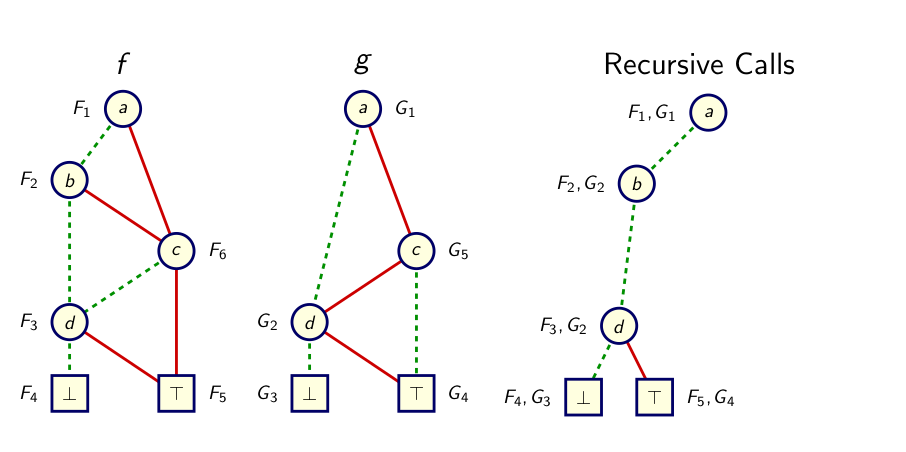
\includegraphics[scale=0.35]{ex4.png}
\end{frame}

\begin{frame}{Logical Operations}
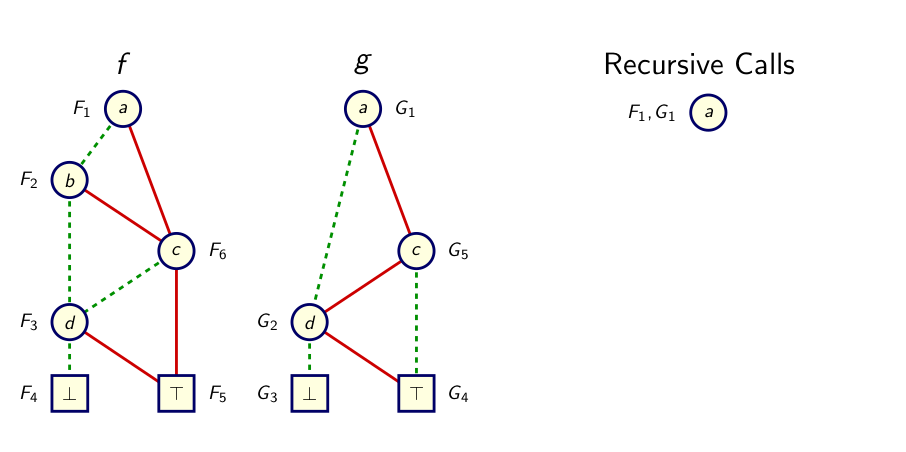
\includegraphics[scale=0.35]{ex1.png}
\end{frame}

\begin{frame}{Logical Operations}
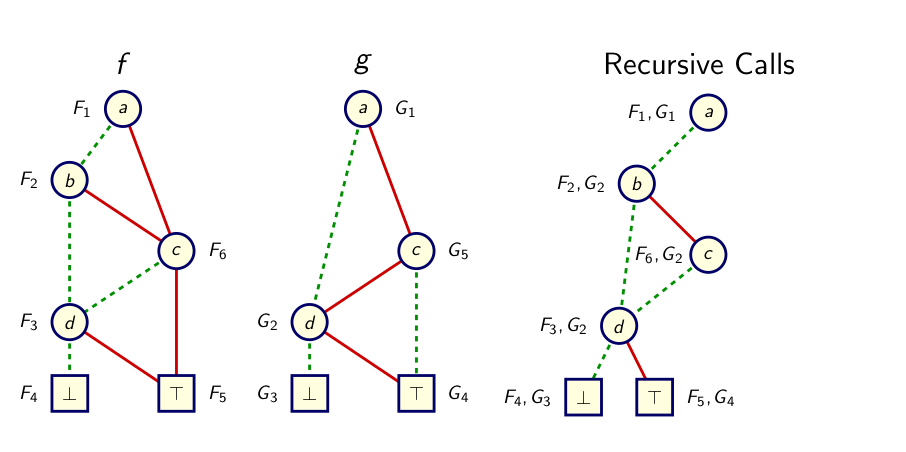
\includegraphics[scale=0.35]{ex5.png}
\end{frame}

\begin{frame}{Logical Operations}
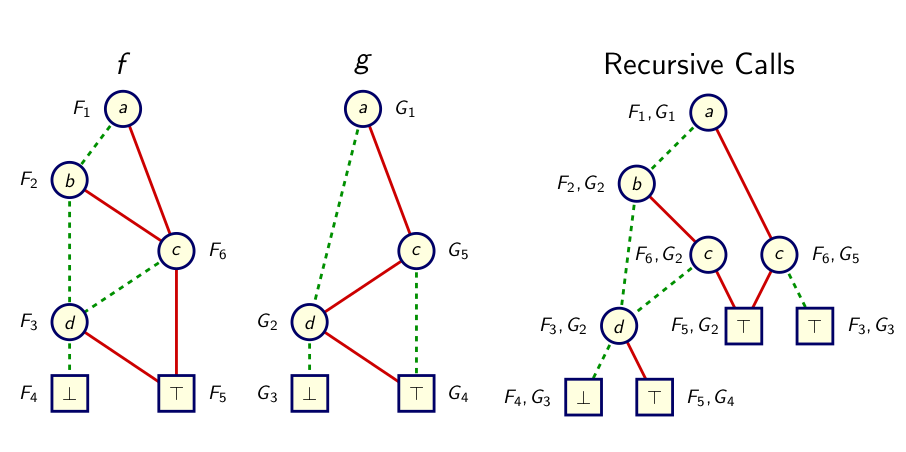
\includegraphics[scale=0.35]{ex6.png}
\end{frame}

\begin{frame}{Logical Operations}
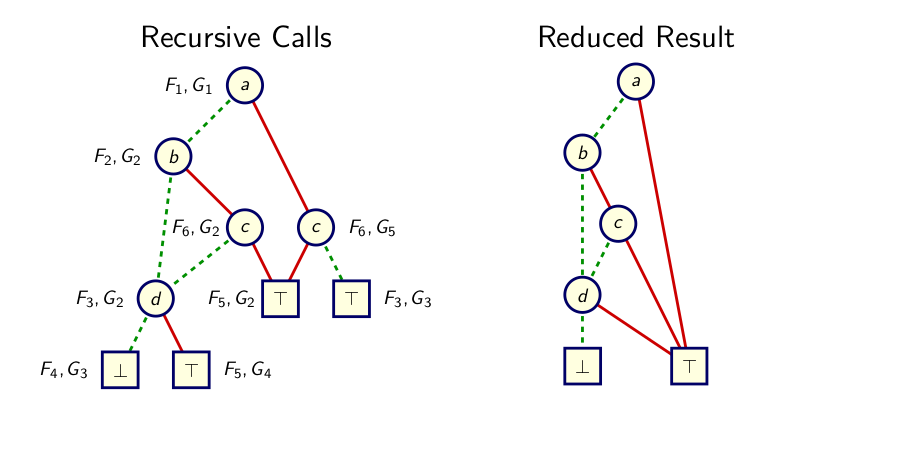
\includegraphics[scale=0.35]{ex7.png}
\end{frame}

\begin{frame}
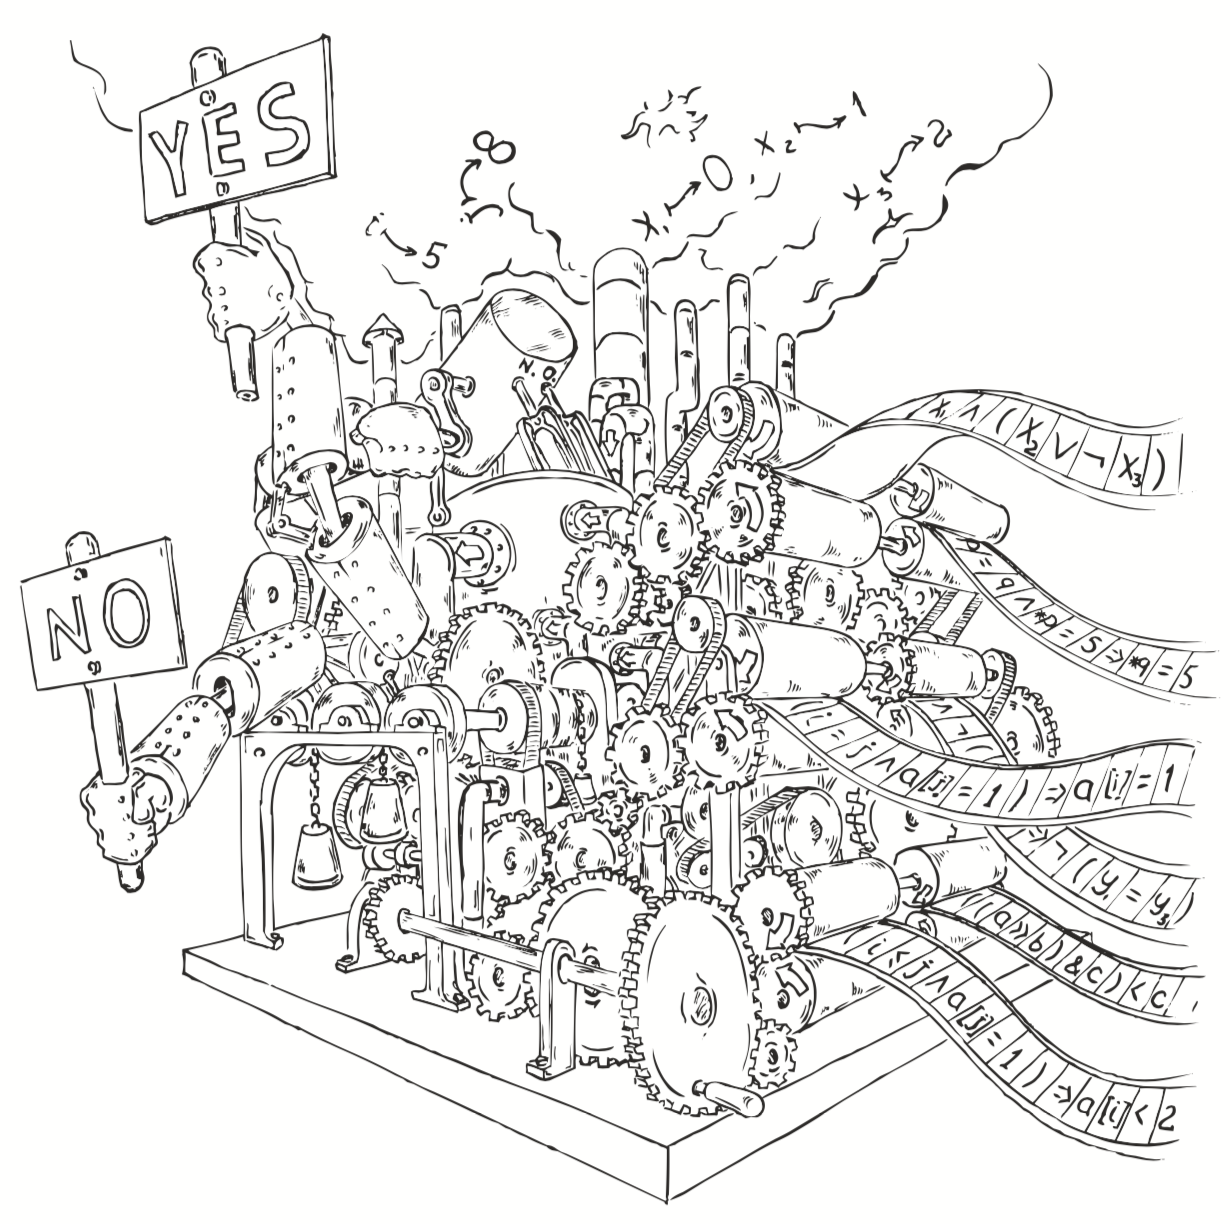
\includegraphics[scale=0.5]{../decision-procedure.png}
\end{frame}

\end{document}
